\documentclass{article}
\usepackage[T1]{fontenc}
\usepackage{lmodern}
\usepackage{graphicx}
\usepackage{amsmath,amssymb}
\usepackage[a4paper,margin=2cm]{geometry}
\usepackage[absolute,overlay]{textpos}
\setlength{\TPHorizModule}{1mm}
\setlength{\TPVertModule}{1mm}
\usepackage[indonesian]{babel}
\usepackage{hyperref}
\setlength{\emergencystretch}{2em}
% unit: Halaman 10

\begin{document}

% === Halaman 10 (llm) ===

\begin{itemize}
    \item Salah satu pekerjaan di dalam \textit{content analysis} adalah mendeteksi apakah ada pesan tersembunyi di dalam sebuah gambar.
    \item Contoh sebuah skenario: Mr. Abdul, seorang investigator forensik, diminta Lab Forensik Polri untuk menginvestigasi sebuah \textit{cybercrime} berupa foto. Sebagai investigator forensik yang ahli, dia menganalisis foto untuk menemukan pesan tersembunyi di dalamnya dengan kakas \underline{steganalisis}.
\end{itemize}
\vspace{10mm}

\vspace{74.84mm}

% deskripsi: Ilustrasi seorang investigator dengan balon teks yang menjelaskan fokus analisis: menemukan konten steganografi dan mengekstrak informasi dari file gambar.
% bbox normalisasi: [0.4820, 0.6160, 0.7480, 0.8680]
\begin{textblock*}{55.86mm}(101.22mm,182.95mm)
\noindent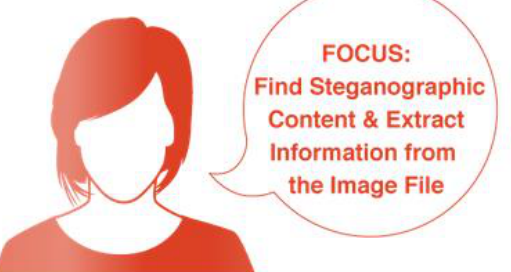
\includegraphics[width=55.86mm,height=74.84mm]{../../images/llm/page_010_img_01.png}%
\end{textblock*}

\end{document}
